\documentclass[11pt, oneside]{article}   	% use "amsart" instead of "article" for AMSLaTeX format


%\usepackage{draftwatermark}
% \SetWatermarkText{Confidential}
% \SetWatermarkScale{5}
% \SetWatermarkLightness {0.85} 
% \SetWatermarkColor[rgb]{0.7,0,0}


\usepackage{geometry}                		% See geometry.pdf to learn the layout options. There are lots.
\geometry{letterpaper}                   		% ... or a4paper or a5paper or ... 
%\geometry{landscape}                		% Activate for for rotated page geometry
%\usepackage[parfill]{parskip}    		% Activate to begin paragraphs with an empty line rather than an indent
\usepackage{graphicx}				% Use pdf, png, jpg, or eps� with pdflatex; use eps in DVI mode
								% TeX will automatically convert eps --> pdf in pdflatex		
\usepackage{amssymb}
\usepackage{mathrsfs}
\usepackage{hyperref}
\usepackage{url}
\usepackage{authblk}
\usepackage{amsmath}
\usepackage{graphicx}
\usepackage{fixltx2e}
\usepackage{hyperref}
\usepackage{alltt}
\usepackage{color}


\title{Notes on Maximization of Inner Products over Norm Balls}
\author{David Meyer \\ dmm@\{1-4-5.net,uoregon.edu,...\}}

\date{March 16, 2017}							% Activate to display a given date or no date


\begin{document}
\maketitle
\begin{abstract}
This document started life as an exploration into the surprising discovery of \emph{adversarial examples} by Szegedy et al. \cite{Szegedy:2013aa}. This discovery has, among other things, led to new ways of thinking about unsupervised training of deep models \cite{NIPS2014_5423} while at the same time causing confusion and concern about the nature of learning in such (deep) models. These notes explore the analysis of adversarial examples given in \cite{Goodfellow:2014aa} and elsewhere. In particular, I couldn't understand why for linear models, the perturbation $\mathbf{w}^{T}\boldsymbol{\eta}$ was maximized by setting $\boldsymbol{\eta} = \text{sign}(\mathbf{w})$. The answer is related to what are called Norm Balls and the relationship between norms and inner products.
\end{abstract}

\section{Introduction} 
\label{sec:intro}

\noindent
The surprising discovery of \emph{adversarial examples} by Szegedy et al. \cite{Szegedy:2013aa} has led to new ways of thinking about unsupervised training of deep models \cite{NIPS2014_5423} while at the same time causing confusion and concern about the nature of learning in such (deep) models. These notes explore the analysis of adversarial examples given in \cite{Goodfellow:2014aa} and elsewhere.

\bigskip
\noindent
What Szegedy et al. \cite{Szegedy:2013aa}  discovered was that several machine learning models, including state-of-the-art neural networks, are vulnerable to adversarial examples. That is, these machine learning models can misclassify examples that are only slightly different (imperceptibly so in many cases)  from correctly classified examples drawn from the data distribution. In many cases, a wide variety of models with different architectures trained on different subsets of the training data misclassify the same adversarial example (this is kind of shocking). The implication is that adversarial examples expose fundamental problems in popular training algorithms.

\section{Linear Explanation of Adversarial Examples}
\label{sec:linear_explanation}
\noindent
In  \cite{Goodfellow:2014aa}, a discussion of the "Linear Explanation of Adversarial Examples"  explains the existence of adversarial examples for linear models. The section starts with a description of the precision of the sensor or storage media. Here they use the example of digital images, which often use only eight bits per pixel (gray scales) and as a result they discard all information below $\frac{1}{255}$ of the dynamic range. The point here is that since the precision of the features is limited,  it makes little sense for a classifier to respond differently to an input $\boldsymbol{x}$ than to an adversarial input $\hat{\boldsymbol{x}}  = \boldsymbol{x} + \boldsymbol{\eta}$, if of course every element of the perturbation $\boldsymbol{\eta}$ is smaller than the precision of the features. Let's say that $\epsilon$ is the largest value \emph{below} the resolution of the sensor (or storage media). Then for problems with well-separated classes, we expect a classifier to assign the same class to $\mathbf{x}$ and
$\hat{\mathbf{x}}$, so long as $||\boldsymbol{\eta}||_{\infty} <  \epsilon$ (where $||\boldsymbol{x}||_{\infty}$ is the \emph{max} or \emph{infinity} norm).

\bigskip
\noindent
Next, consider the activation induced by an adversarial example $\hat{\mathbf{x}}$:

\begin{flalign}
\hat{\mathbf{x}}  &= \mathbf{x} + \boldsymbol{\eta}   \quad \qquad \qquad \qquad  \mathbin{\#} \text{adversarial example } \hat{\mathbf{x}}  \text{ given perturbation } \boldsymbol{\eta} \\
\mathbf{w}^{\text{T}}\hat{\boldsymbol{x}}  &= \mathbf{w}^{\text{T}}\boldsymbol{x} + \mathbf{w}^{\text{T}} \boldsymbol{\eta} \qquad \qquad  \mathbin{\#} \text{activation } \mathbf{w}^{\text{T}}\hat{\boldsymbol{x}} \text{ induced by } \boldsymbol{\eta}
\end{flalign}

\bigskip
\noindent
\textbf{Notes:} 
\noindent
\begin{itemize}
\item The adversarial perturbation causes the activation to grow by $\mathbf{w}^{\text{T}} \boldsymbol{\eta}$
\item $\mathbf{w}^{\text{T}} \boldsymbol{\eta}$  is maximized, subject to $||\boldsymbol{\eta}||_{\infty} < \epsilon$, by assigning  $\boldsymbol{\eta} =  \text{sign}(\boldsymbol{w})$ 
\end{itemize}


\bigskip
\noindent
What I couldn't understand about Goodfellow's description is why, in the linear case, the perturbation $\mathbf{w}^{\text{T}} \boldsymbol{\eta}$  is maximized, subject to $||\boldsymbol{\eta}||_{\infty} < \epsilon$, by assigning  $\boldsymbol{\eta} =  \text{sign}(\boldsymbol{w})$, where the sign or signum function is defined at follows:

\begin{flalign*}\text{sign}(x)  :=
\left \{ 
        \begin{array}{rr}
		-1   & \text{if } x < 0 \\
		0    & \text{if } x = 0 \\
		1    & \text{if } x > 0
	\end{array}
\right.
\end{flalign*}

\bigskip
\noindent
The remainder of this note contains a brief overview of 
the \emph{Maximization of Inner Products over Norm Balls}, which contains the parts of the answer to my question.


\section{The Maximization of Inner Products over Norm Balls}
First, what is a norm? The most common definition involves a function $||.||: \mathbb{R}^n \rightarrow \mathbb{R}$, the \emph{vector norm}, which has the following properties:

\begin{enumerate}
\item $||\textbf{x}|| \geq 0$ for any vector $\mathbf{x} \in \mathbb{R}^n$, and $||\textbf{x}|| = 0$ iff $\textbf{x} = 0$
\item $||\alpha \mathbf{x}|| = |\alpha| ||\mathbf{x}||$  for any vector $\mathbf{x} \in \mathbb{R}^n$ and any scalar $\alpha$
\item $||\mathbf{x} + \mathbf{y}|| \leq ||\mathbf{x}|| + ||\mathbf{y}||$ for any vectors $\mathbf{x},\mathbf{y} \in \mathbb{R}^n$
\end{enumerate}
\noindent
The last property is called the \emph{triangle inequality}. Note also that when $n = 1$, the absolute
value function is a vector norm. 

\bigskip
\noindent
The most commonly used vector norms belong to the family of $l$-norms, or sometimes $l_p$-norms, which
are defined as

\begin{flalign}
||\mathbf{x}||_{p} = \Big(\sum\limits_{i=1}^{n} |x_i|^p\Big)^{\frac{1}{p}}
\end{flalign}

\begin{figure}
\center{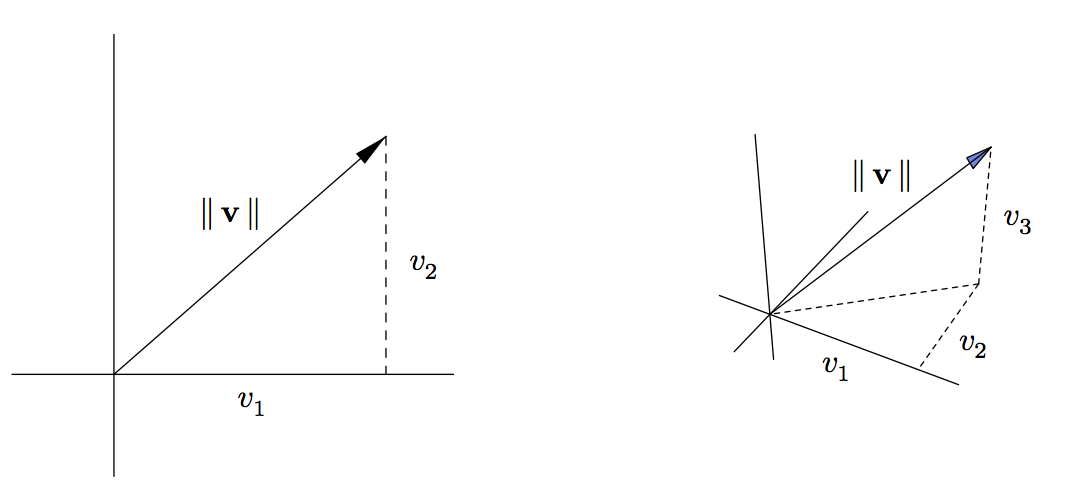
\includegraphics[scale=0.8] {images/euclidean_norm.png}}
\caption{Euclidean Norms in $\mathbb{R}^2$ and  $\mathbb{R}^3$}
\label{fig:euclidean_norms}
\end{figure}

\bigskip
\noindent
Now,  it can be shown that for any $p > 0$, $||.||_p$ defines a vector norm. The vector norms of particular interest include:
\begin{itemize}
\item $p = 1$:  The $\ell_1$-norm $||\mathbf{x}||_1 = \sum\limits_{i=1}^n |x_i|$
\item $p = 2$:  The $\ell_2$-norm or \emph{Euclidean} norm $||\mathbf{x}||_2 = \sqrt{\sum\limits_{i=1}^n  x^2_i} = \sqrt{\mathbf{x}^{\text{T}}\mathbf{x}}$
\item $p = \infty$: The $\ell_\infty$-norm $||\mathbf{x}||_\infty = \max\limits_{1 \leq i \leq n} |x_i|$
\end{itemize}

\bigskip
\noindent
Figure \ref{fig:euclidean_norms} shows the Euclidean Norms in $\mathbb{R}^2$ and  $\mathbb{R}^3$.


\bigskip
\noindent
There are many (many) useful theorems one can prove here, but I want to jump ahead to norm balls.

\subsection{What is a Norm Ball?}
Again there are many theorems one can prove about norm balls, but suffice it to say that in Cartesian space $\mathbb{R}^n$ with the $p$-norm, $\ell_p$, an open ball is the set
\begin{flalign}
B(r) = \Big\{\mathbf{x} \in \mathbb{R}^n : \sum\limits_{i=1}^n |x_i|^p < r^p\Big\} \qquad \qquad  \mathbin{\#} r \text{ is the radius of ball $B$}
\end{flalign}

\bigskip
\noindent
For $n = 2$, in particular, the balls of $\ell_1$ (often called the taxicab or Manhattan metric) are squares with the diagonals parallel to the coordinate axes; those of $\ell_\infty$  (the Chebyshev metric) are squares with the sides parallel to the coordinate axes. For other values of $p$, the balls are bounded by Lam� curves (hypoellipses or hyperellipses). For $n = 3$, the balls of $\ell_1$ are octahedra with axis-aligned body diagonals, those of $\ell_\infty$ are cubes with axis-aligned edges, and those of $\ell_p$ with $p > 2$ are superellipsoids. See Figure \ref{fig:norm_ball} for a few examples.

\begin{figure}
\center{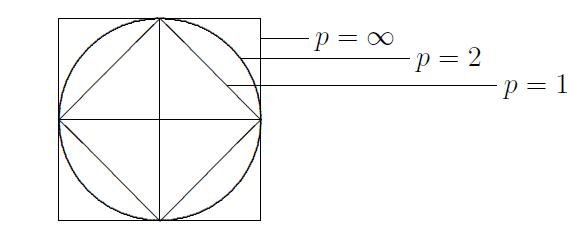
\includegraphics[scale=0.8] {images/norm_ball.png}}
\caption{Norm Balls in $\mathbb{R}^2$}
\label{fig:norm_ball}
\end{figure}


\section{Maximization of Inner Products over Norm Balls}
Finally we're getting to the heart of the matter. There is an interesting relationship between inner products and norms, but I'm going to skip that here. Rather, consider the following: Given a nonzero vector $\mathbf{y} \in \mathbb{R}^n$,, consider the problem of finding some vector $\mathbf{x} \in \mathcal{B}_p$ (i.e., the unit ball in $\ell_p$ norm) that maximizes the inner product $\mathbf{x}^{\text{T}}\mathbf{y}$. That is, given some nonzero vector $\mathbf{y}$, we want to solve for $\mathbf{x}$ that satisfies 
$\max\limits_{|| \mathbf{x}||_p  \leq 1}\mathbf{x}^{\text{T}}\mathbf{y}$.


\bigskip
\noindent
For $p = 2$, the solution is straight forward since 
$\mathbf{x}^{\text{T}}\mathbf{y} = \cos \theta ||\mathbf{x}||_2 || \mathbf{y} ||_2$; $\mathbf{x}$ should be parallel to $\mathbf{y}$ (i.e., the angle between $\mathbf{x}$ and $\mathbf{y}$ is zero) so that the norm is as large as possible, that is, one. The unique solution is here is $\mathbf{x}^*_2 = \frac{\mathbf{y}}{||\mathbf{y}||_2}$.

\bigskip
\noindent
This is where things get (more) interesting and relevant to my question as to why $\boldsymbol{\eta}$ is set to $\text{sign}(\mathbf{w})$ in Goodfellow's work.  So consider the case where $p = \infty$, i.e., the max norm. Now, 
since $\mathbf{x}^{\text{T}}\mathbf{y} = \sum\limits_{i=1}^n x_iy_i$, where each element $x_i$ is such that $|x_i| \leq 1$, \textcolor{red}{we can see that the sum is maximized by setting $x_i = \text{sign}(y_i)$}. Further, we can see that 
$\max\limits_{||\mathbf{x}||_\infty \leq 1}\mathbf{x}^{\text{T}}\mathbf{y}  = \sum\limits_{i=1}^n |y_i| = ||\mathbf{y}||_1$. So here we see that the optimal solution may not be unique, since any $x_i \in [-1,1]$, corresponding to $y_i = 0$, could be selected without modifying the optimal value. 

\bigskip
\noindent
Finally, for completeness, consider the case where $p = 1$. Here the inner product $\mathbf{x}^{\text{T}}\mathbf{y} = \sum\limits_{i=1}^n x_iy_i$ can be interpreted as a weighted average of the $y_i$'s where the $x_i$'s are the weights whose absolute values must sum up to one. The maximum of the weighted average is achieved by first finding the $y_i$ having the largest absolute value, that is, by finding one index $m$ such that $|y_i| \leq |y_m|$ for all $i = 1, 2, \cdots,n$, and then setting 

\begin{flalign*}|x^*_1|_i =
\left \{ 
        \begin{array}{ll}
		\text{sign}(y_i) & \text{if } i = m \\
		0                      & \text{otherwise}
	\end{array}
\right.
\end{flalign*}

\bigskip
\noindent
What we wind up with there is that $\max\limits_{||\mathbf{x}||_1 \leq 1} \mathbf{x}^{\text{T}}\mathbf{y} = \max_i |y_i| = ||\mathbf{y}||_\infty$. Here again the optimal solution may not be unique since in the case when $\mathbf{y}$ has more than one entry with maximum absolute value we can choose $m$ to be any of the indicies corresponding to these maxima.  This shows the goal of maximizing inner products over norm balls, namely to create a n-dimensional unit vector that goes from the origin to the surface of the norm ball.

\newpage
\bibliographystyle{acm}
% \bibliographystyle{plain}
\bibliography{/Users/dmm/papers/bib/ml}



\end{document} 
